\documentclass{beamer}
\usetheme{STCE}
\usepackage{beamerfoils}
\usepackage{listings}

% Setze Codesprache auf C
\lstset{language=C}

\MyLogo{
\centering

\includegraphics[width=0.12\textwidth]{./figures/logo.eps}
}

\begin{document}
\title{Correlation and Regression Analysis}
\author{Patrick Neidig \and Marius Grysla}
\institute{Software and Tools for Computational Engeneering}
\date{19.4.2011}
\frame{\titlepage}

%%%%% Überblick %%%%%
\begin{frame}
 \frametitle{\"Uberblick}
 \tableofcontents
\end{frame}

%%%%% Alternativen %%%%%
\section{Alternativen}

\begin{frame}
 \frametitle{Alternativen}
 \begin{itemize}
  \item GSL (GNU Scientific Library)
   \begin{itemize}
    \item numerische Bibliothek f\"ur C und  C++
    \item frei unter GNU-Lizenz erh\"altlich
   \end{itemize}
  \item IMSL (International Mathematics and Statistics Library)
   \begin{itemize}
    \item kommerzielle numerische Bibliothek f\"ur Fortran, C, C\#.NET, Java und Python
   \end{itemize}
  \item R Project for Statistical Computing
  \begin{itemize}
    \item freie Software zur statischen Berechnung und Darstellung
   \end{itemize}
 \end{itemize}

\end{frame}

%%%%% Anwendungsbereiche %%%%%
\begin{frame}
 \frametitle{Anwendungsbereiche}

 \begin{itemize}
  \item Wirtschaft
  \begin{itemize}
   \item Wie effektiv ist eine Werbungskampagne?
  \end{itemize}

  \item Medizin
  \begin{itemize}
   \item Wie h\"angen bestimmte Merkmale mit Krankheiten zusammen?
  \end{itemize}

  \item Sozialwissenschaften
  \begin{itemize}
   \item Kann von der H\"ohe des Einkommens auf den Besitz eines Autos geschlossen werden?
  \end{itemize}


 \end{itemize}

\end{frame}

%%%%% Korrelation %%%%%
\section{Korrelation}

\begin{frame}
	
	\frametitle{Korrelation}
	
	\begin{itemize}
		
		\item bi-/multivariate Statistik
		\begin{itemize}
			\item gleichzeitige Analyse zweier bzw. mehrerer Merkmale statistischer Objekte (z.B. Personen)
			\item Merkmal $X$ mit Merkmalsauspr\"agungen $x_1, x_2, ..., x_m$ sowie Merkmal $Y$ mit Merkmalsauspr\"agungen $y_1, y_2, ..., y_n$ (z.B. K\"orpergr\"o\ss e und Gewicht von Personen)
		\end{itemize}
		
		\item Streudiagramm
		\begin{itemize}
			\item graphische Darstellung aller auftretenden Merkmalspaare $(x_i,y_j)$ als Punkte im zweidimensionalen Koordinatensystem
		\end{itemize}

		\item Korrelation
		\begin{itemize}
			\item St\"arke des Zusammenhangs von Merkmalen
			\item mit Hilfe verschiedener Korrelationskoeffizienten messbar
		\end{itemize}
		
	\end{itemize}
	
\end{frame}

\begin{frame}
	
	\frametitle{Korrelationskoeffizienten}
	
	\begin{itemize}
		
		\item Korrelationskoeffizient nach Bravais und Pearson
		\begin{itemize}
			\item misst linearen Zusammenhang von Merkmalen
			\item f\"ur mind. intervallskalierte Merkmale
		\end{itemize}
		
		\item Rangkorrelationskoeffizienten 
		\begin{itemize}
			\item messen monotonen Zusammenhang von Merkmalen
			\item f\"ur mind. ordinalskalierte Merkmale
			\item Umwandlung der Merkmalsauspr\"agungen in R\"ange
			\item nach Spearman (Spearmans Rho)
			\begin{itemize}
				\item genaue Berechnung der Rangdifferenzen
			\end{itemize}
			\item nach Kendall (Kendalls Tau)
			\begin{itemize}
				\item einfache Anordnung der R\"ange
			\end{itemize}
		\end{itemize}

		\item f\"ur Korrelationskoeffizienten $r$ gilt allgemein $-1 \leq r \leq +1$
				
	\end{itemize}
	
\end{frame}

\begin{frame}
	
	\frametitle{Beispiele}
	
	\centering
 		\only<1>{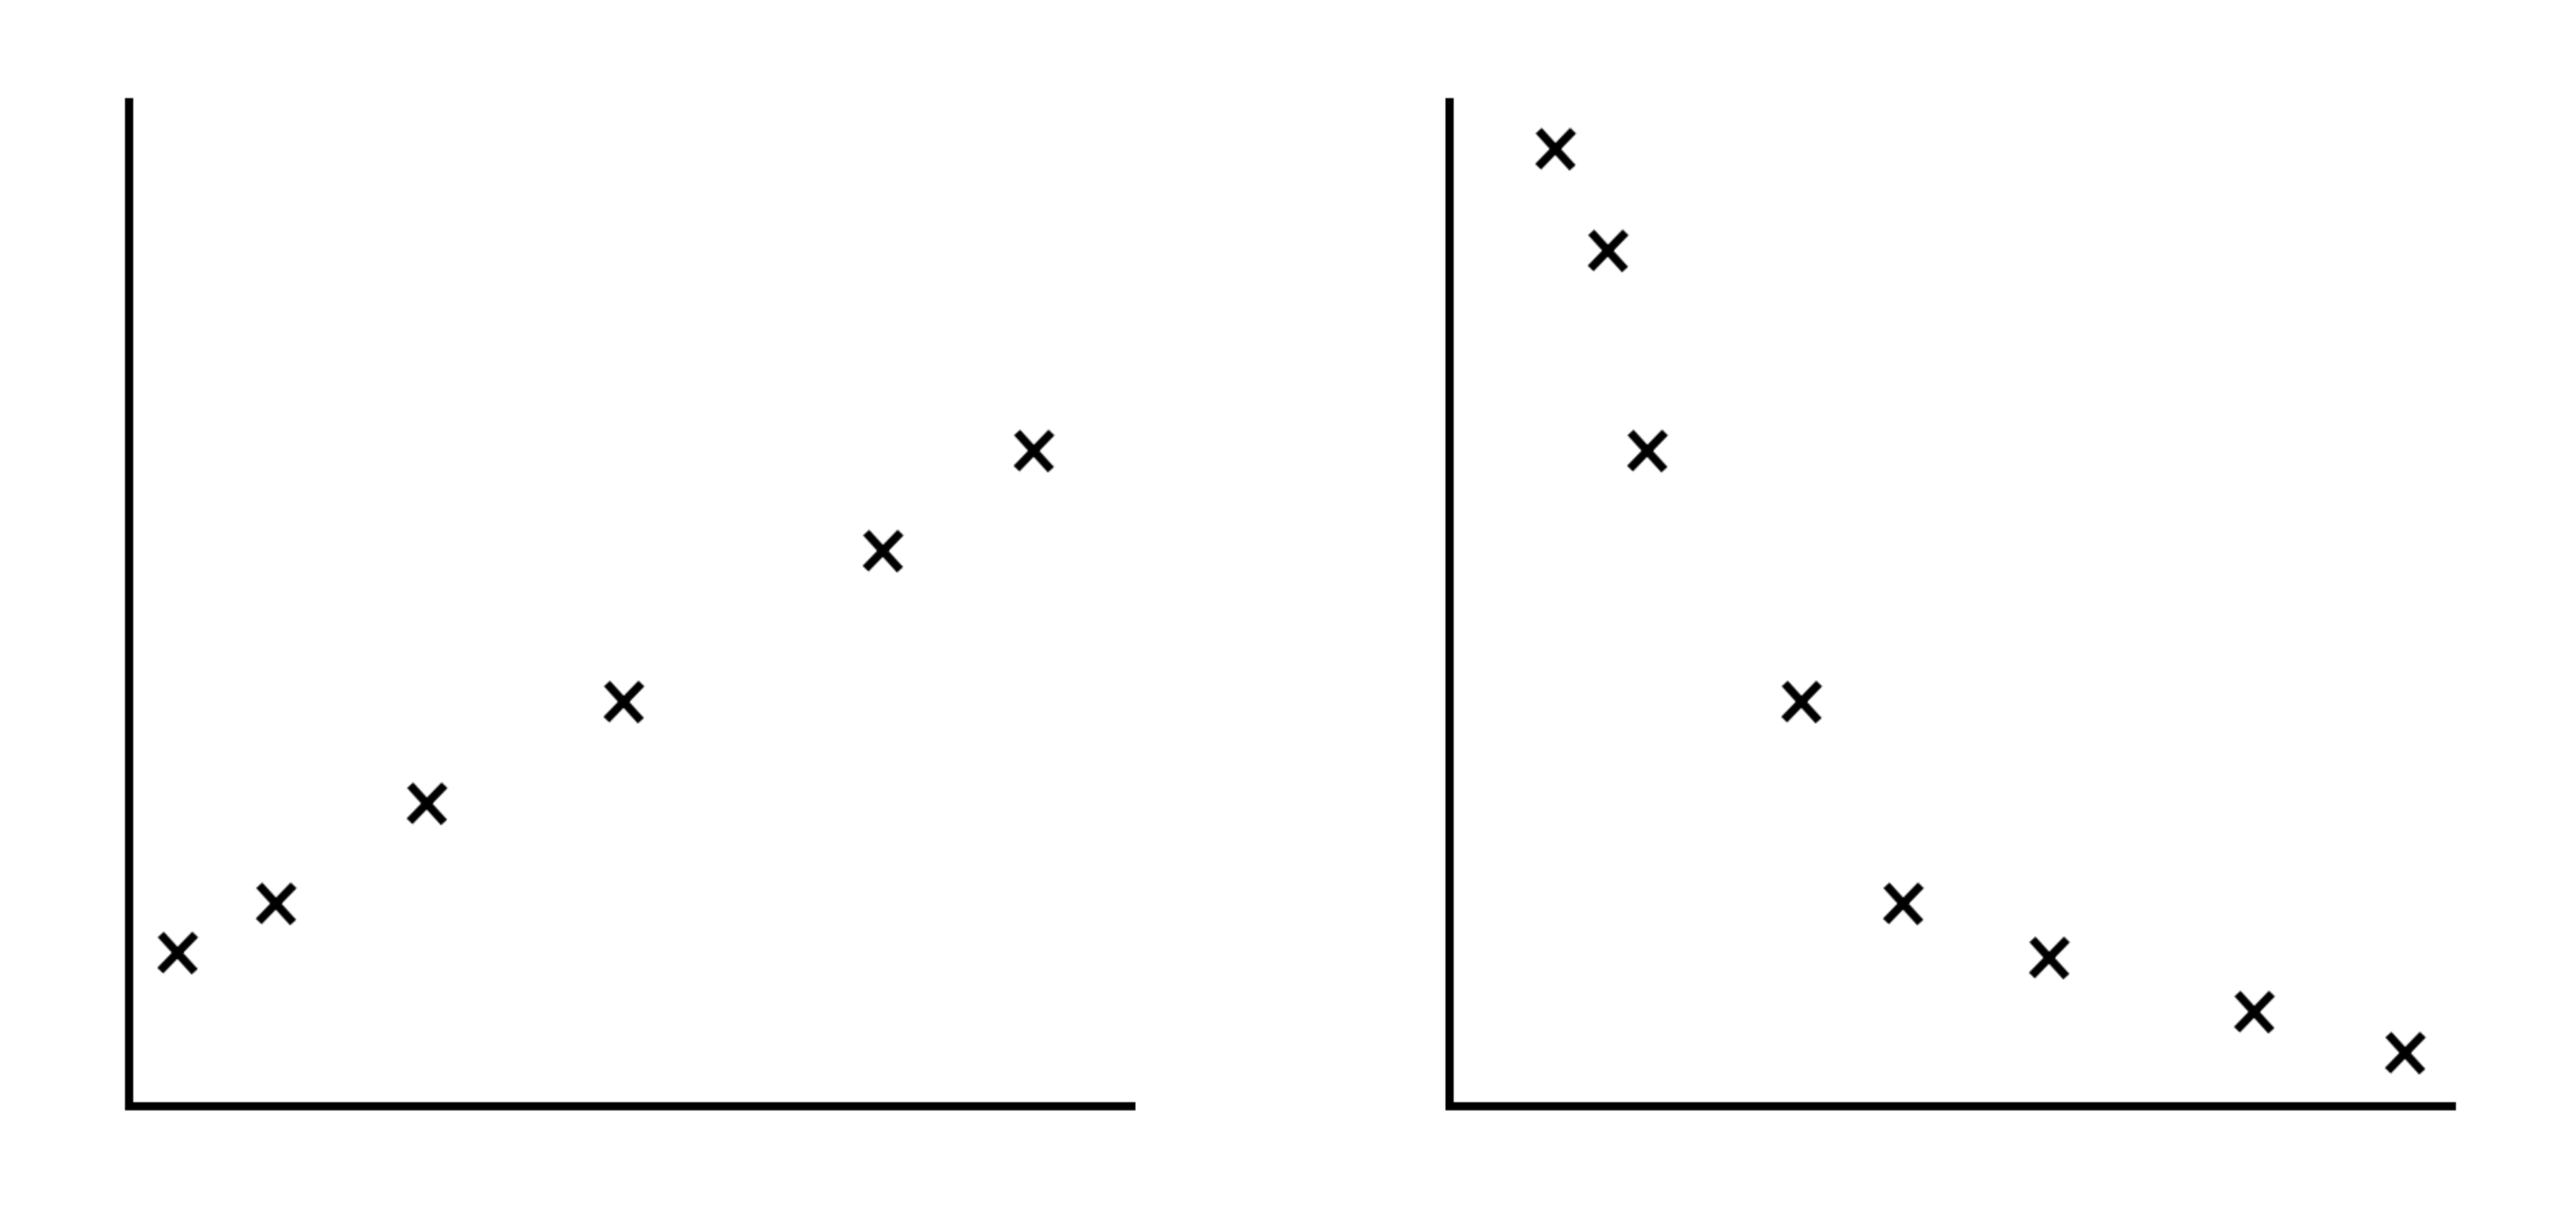
\includegraphics[width=10cm]{./figures/streudiagramme.eps}}%
	
\end{frame}

\begin{frame}
	
	\frametitle{Partielle Korrelation}
	
	\begin{itemize}
		
		\item Korrelation ist kein Beleg f\"ur kausalen Zusammenhang
		
		\item Scheinkorrelation
		\begin{itemize}
			\item scheinbare Korrelation zwischen Merkmalen $X$ und $Y$ (z.B. K\"orpergr\"o\ss e und Wortschatz von Kindern) kann unter Umst\"anden auf Einfluss eines zus\"atzlichen Merkmals $Z$ (z.B. Alter) zur\"uckgef\"uhrt werden
		\end{itemize}
		
		\item \"Uberpr\"ufung durch partielle Korrelation
		
	\end{itemize}
	
\end{frame}

\begin{frame}

	\frametitle{Einige NAG-Funktionen zur Korrelation}
 
	\begin{itemize}

		\item \alert<2>{Korrelationskoeffizient nach Bravais und Pearson: \hfill \lstinline{nag\_corr\_cov}}
		\begin{itemize}
			\item berechnet Korrelationsmatrix
		\end{itemize}
		
		\item \alert<2>{Rangkorrelationskoeffizienten: \hfill \lstinline{nag\_ken\_spe\_corr\_coeff}}

		\item \alert<2>{Partielle Korrelation: \hfill \lstinline{nag\_partial\_corr}}
		\begin{itemize}
			\item verwendet Korrelationsmatrix von nag\_corr\_cov
		\end{itemize}
		
		\item Robuste Korrelation: \hfill \lstinline{nag\_robust\_corr\_estim}
		\begin{itemize}
			\item reduziert den Einfluss von "Ausrei\ss ern"
		\end{itemize}

	\end{itemize}

\end{frame}

%%%%% Regressions Analyse %%%%%
\section{Regressions Analyse}

\begin{frame}
 \frametitle{Regression}
 
 \begin{block}{Ziel}
  Darstellung des Verh\"altnisses zwischen zwei Variablen als Funktion:\\
  \centering $Y = a + bX + \epsilon$
 \end{block}


 \begin{itemize}
  \item Grundlage: Beobachtete Messreihe $(x_1, y_1), \dots, (x_n, y_n)$
 \end{itemize}

 \pause

 \begin{block}{Methode der kleinsten Quadrate}
  \centering
  \only<1-2>{$Q(f) = \sum\limits_{i=1}^{n} (y_i - f(x_i))^2 = \sum\limits_{i=1}^{n} \epsilon_i^2 \rightarrow min$}
  \only<3->{$Q($\alert<3>{$a, b$}$) = \sum\limits_{i=1}^{n} (y_i - $\alert<3>{$(a + bx_i)$}$)^2 = \sum\limits_{i=1}^{n} \epsilon_i^2 \rightarrow min$}\\
  \only<4>{$\widehat{a} = \overline{y} - \widehat{b} \overline{x}$\\~\\}
  \only<4>{$\widehat{b} = \frac{\frac{1}{n} \sum\limits^n_{i=1} x_i y_i - \overline{x} \cdot \overline{y}}{\frac{1}{n} \sum\limits^n_{i=1} x_i^2 - \overline{x}^2}$}
  %\only<4>{$\widehat{b} = \frac{\frac{1}{n} \sum\limits^n__{i=1} x_i y_i - \overline{x} \cdot \overline{y}}{\frac{1}{n} \sum\limits^n_{i=1} x_i^2 - \overline{x}^2}$}
 \end{block}

 


\end{frame}

\begin{frame}
 \frametitle{Regressionsbeispiel 1}

 \begin{itemize}
  \item Eine Firma hat in den letzten Monaten mehrere Werbungskampagnen mit unterschiedlichem Aufwand durchgef\"uhrt.
  \begin{itemize}
   \item Steigt der Umsatz mit h\"oherem Aufwand?
   \item Wieviel Werbung ist f\"ur ein Umsatzziel n\"otig?
  \end{itemize}

 \end{itemize}

 \pause
  
 \begin{figure}
    \begin{tabular}{ccccccc}
      \hline
      Monat	& 1	& 2	& 3	& 4	& 5	& 6	\\
      \hline
      Kosten	& 23	& 15	& 43	& 45	& 30	& 51	\\
      Umsatz	& 2,3	& 1,1	& 2,7	& 2,9	& 2,1	& 3,3	\\ 
      \hline
    \end{tabular}
    \caption{Kosten und Umsatz der bisherigen Kampagnen.}
 \end{figure} 

\end{frame}

\begin{frame}
 \frametitle{Regressionsbeispiel 2}

 \centering
  \only<1>{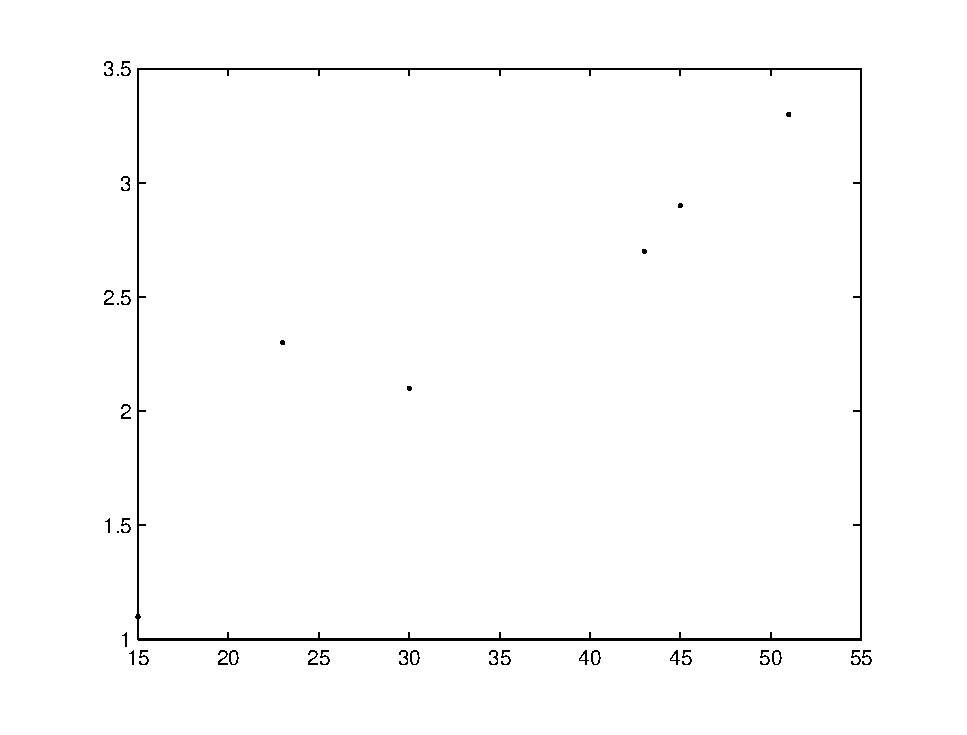
\includegraphics[width=10cm]{./figures/ad-plot-1.eps}}%
  \only<2>{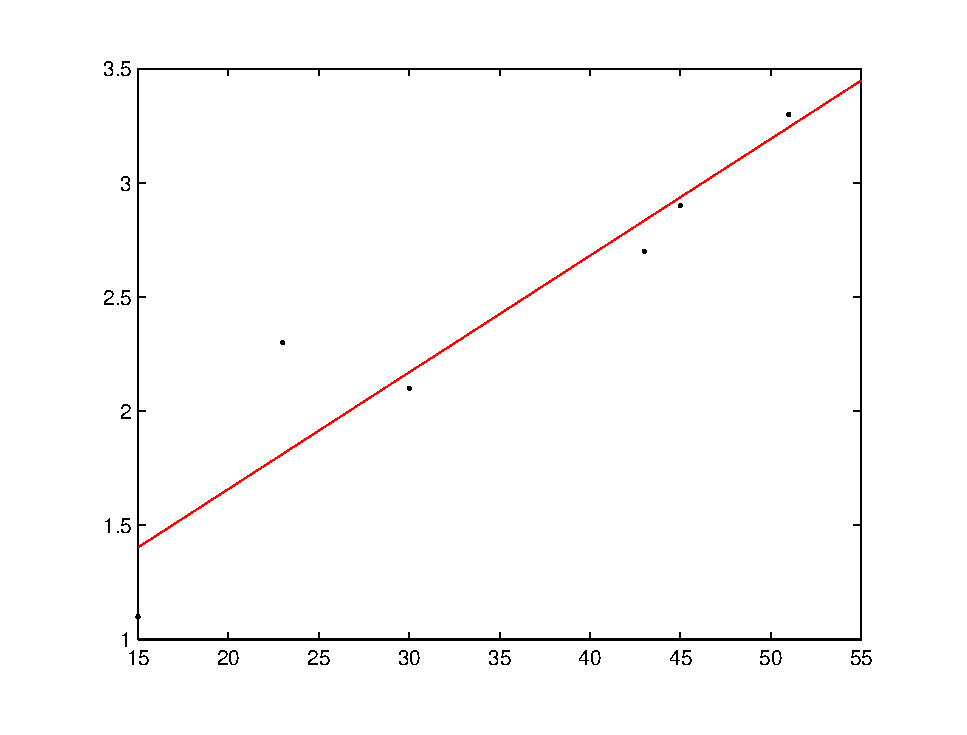
\includegraphics[width=10cm]{./figures/ad-plot-2.eps}}%
  \only<3>{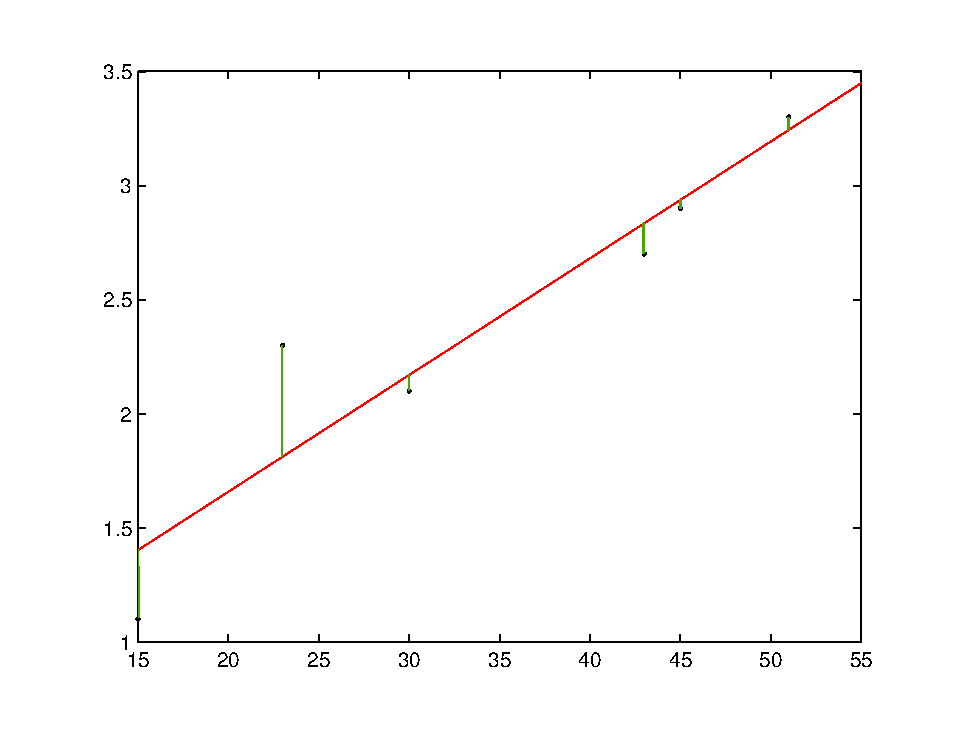
\includegraphics[width=10cm]{./figures/ad-plot-3.eps}}%

\end{frame}

\begin{frame}
 \frametitle{Analyse}
 \begin{itemize}
  \item M\"ogliche Probleme:
  \begin{itemize}
   \item Die Variablen k\"onnten unkorreliert sein
   \item Oft reicht lineare Regression nicht aus
  \end{itemize}

  \item Fehlererkennung
  \begin{itemize}
   \item Korrelationskoeffizient
   \item T-Tests
   \item F-Tests
   \item Varianzen
  \end{itemize}

 \end{itemize}

\end{frame}

\begin{frame}
 \frametitle{Einige NAG Regressions Funktionen}
 \begin{itemize}
  \item \alert<2>{Einfache Lineare Regression: \hfill \lstinline{nag\_simple\_linear\_regression}}	
  \item \alert<2>{Multiple Lineare Regression: \hfill \lstinline{nag\_regsn\_mult\_linear}}
    \begin{itemize}
     \item Mehrere unabh\"angige Variablen
    \end{itemize}
  \item \alert<2>{Robuste Regression: \hfill \lstinline{nag\_robust\_m\_regsn\_user\_fn}}
    \begin{itemize}
     \item Weniger Einflu\ss~ von einzelnen Ausrei\ss ern
    \end{itemize}
  \item Allgemeinere Regression: \hfill \lstinline{nag\_glm\_normal}
    \begin{itemize}
     \item Mehr Flexibilit\"at f\"ur den Benutzer
    \end{itemize}
  \item Ridge Regression \hfill \lstinline{nag\_regsn\_ridge\_opt}
    \begin{itemize}
      \item Wenn Regressoren correliert sind
    \end{itemize}

 \end{itemize}

\end{frame}


%%%%% Zeitplan %%%%%
\section{Zeitplan}

\begin{frame}
 \frametitle{Zeitplan}	
 
 \centering
  \only<1>{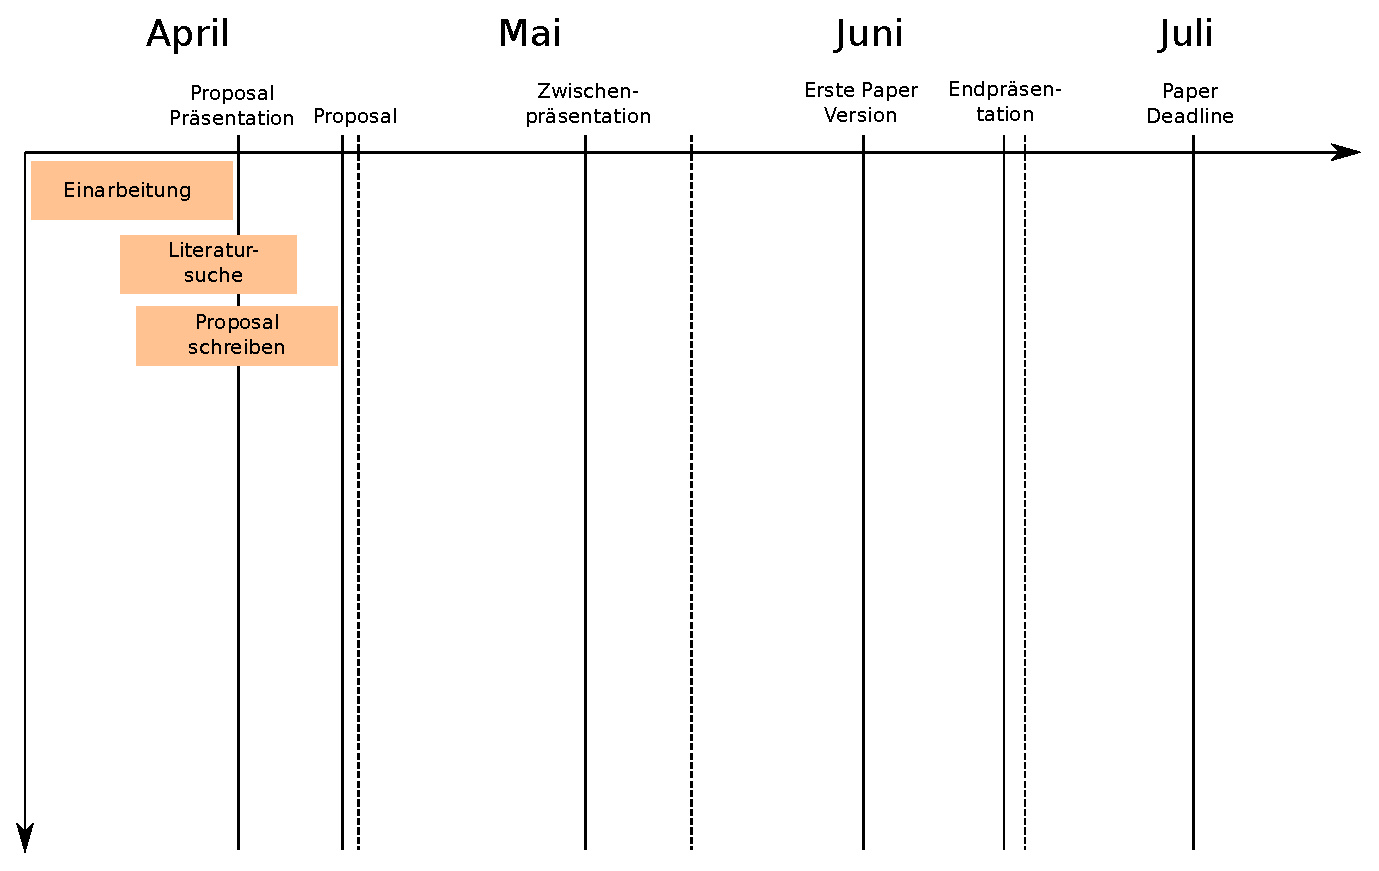
\includegraphics[width=10cm]{./figures/Workplan-adj-1.eps}}%
  \only<2>{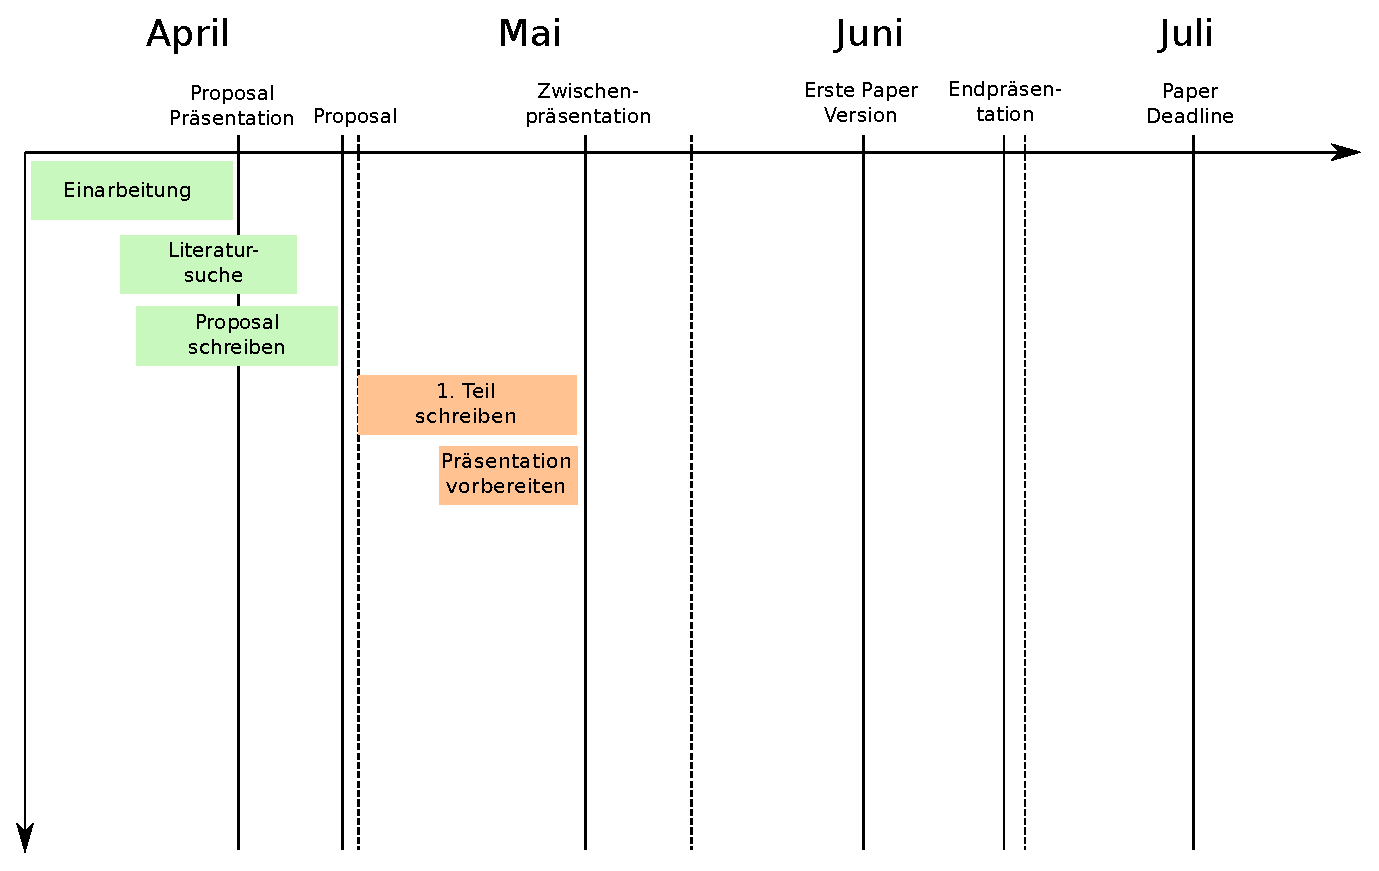
\includegraphics[width=10cm]{./figures/Workplan-adj-2.eps}}%
  \only<3>{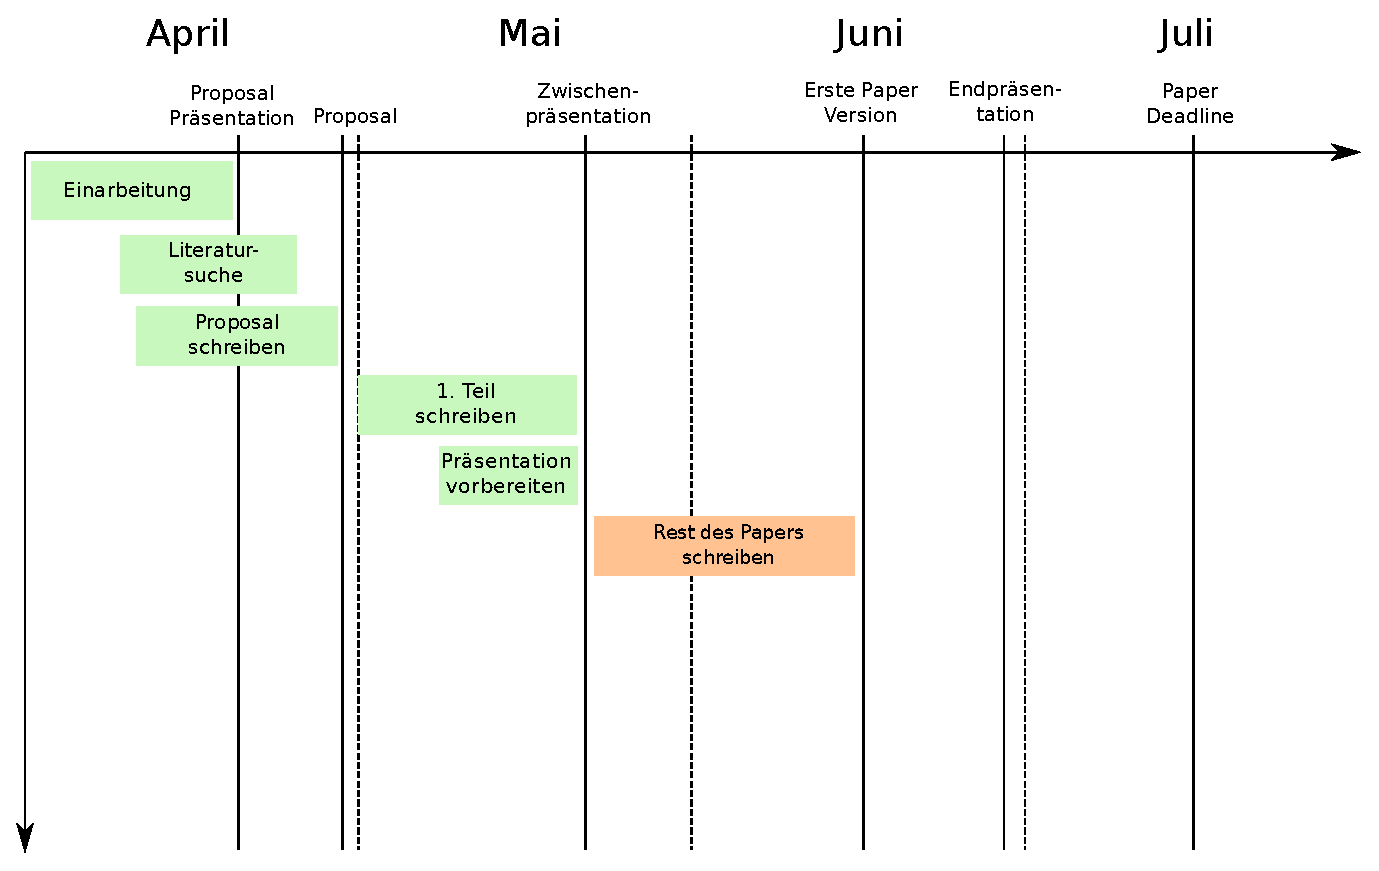
\includegraphics[width=10cm]{./figures/Workplan-adj-3.eps}}%
  \only<4>{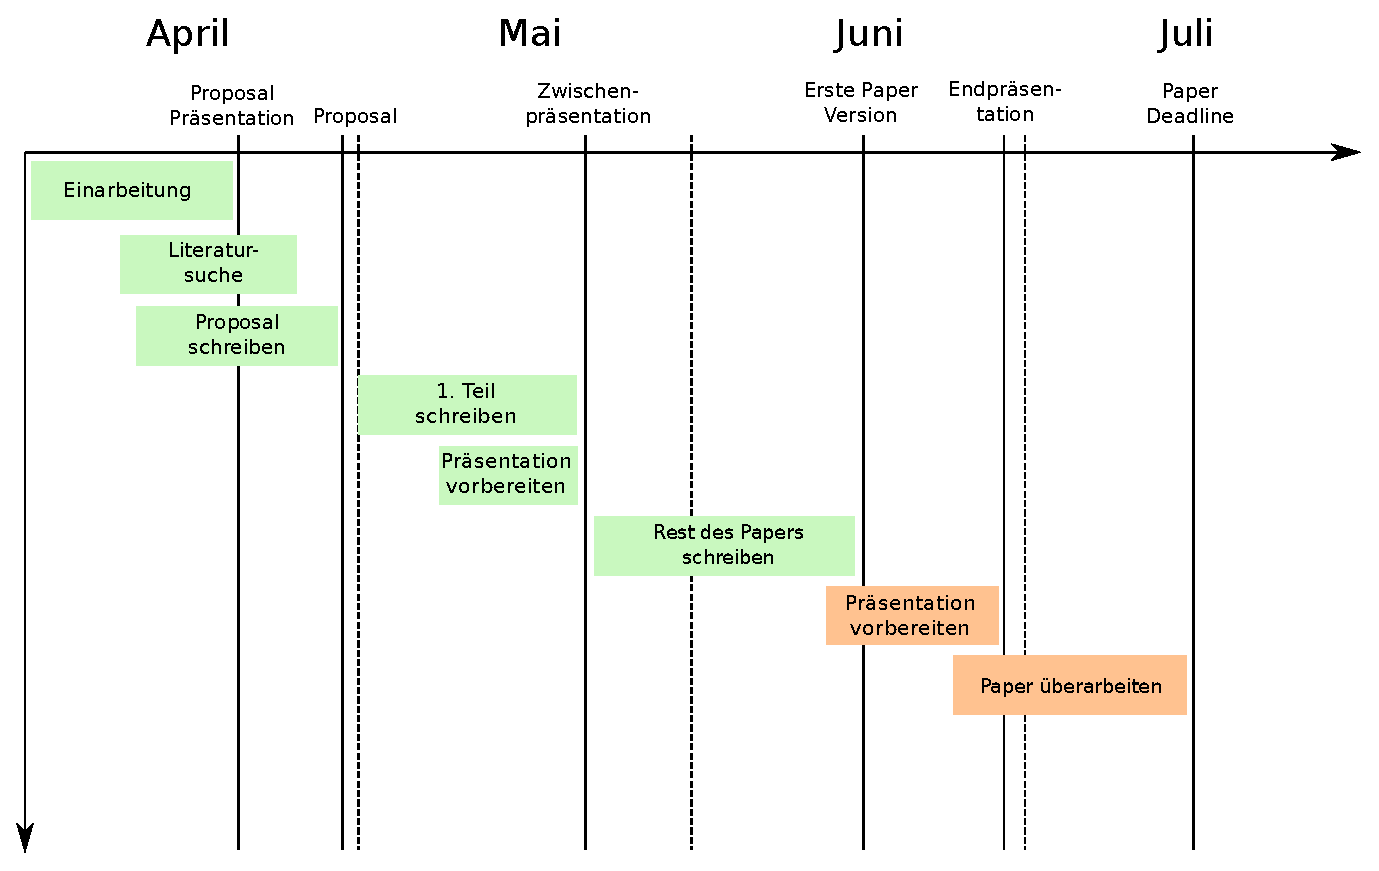
\includegraphics[width=10cm]{./figures/Workplan-adj-4.eps}}%
  \only<5->{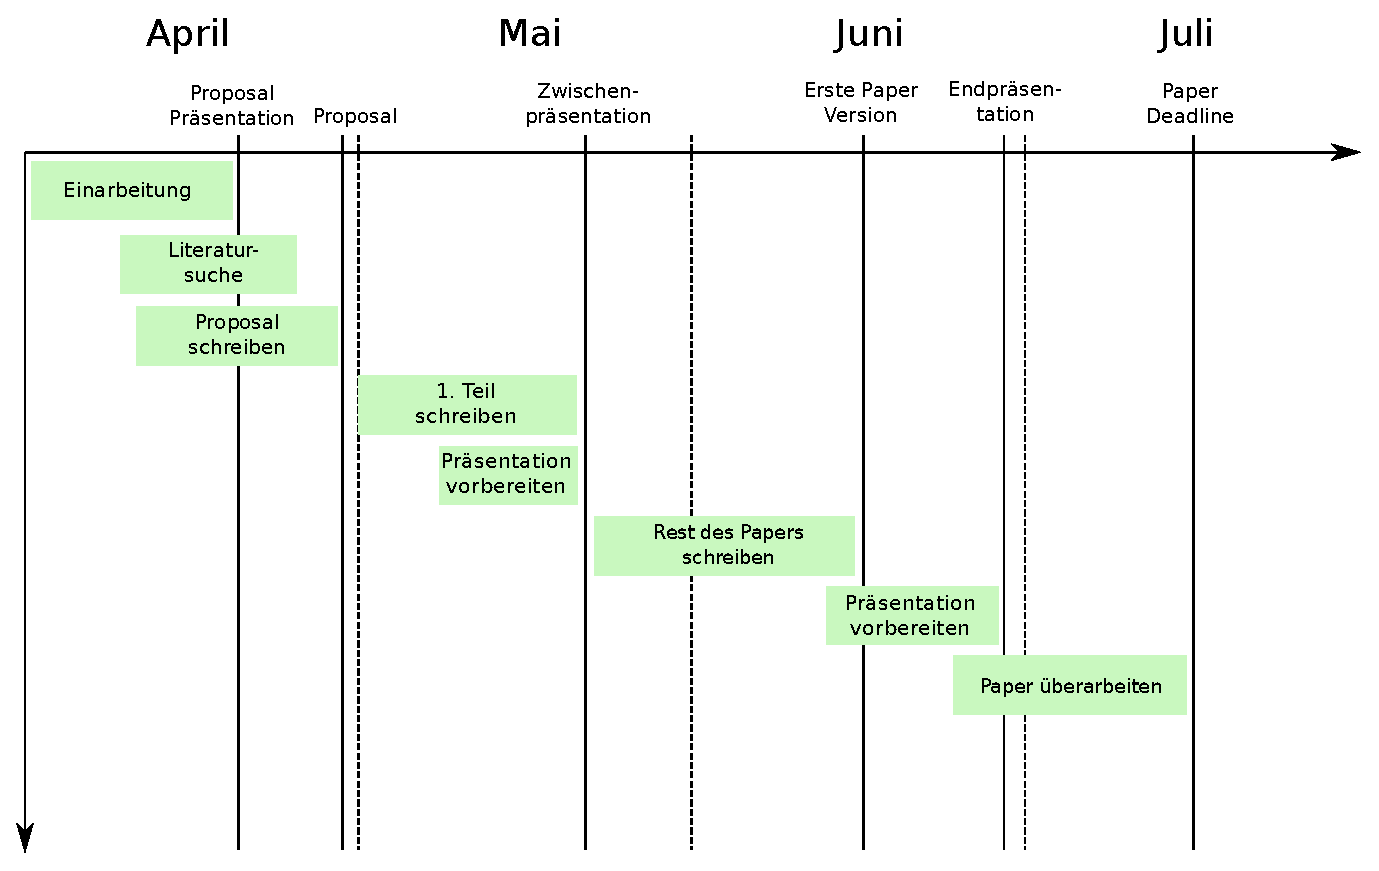
\includegraphics[width=10cm]{./figures/Workplan-adj.eps}}%	

 \begin{itemize}
  \item<5> Kein Notfallplan!
 \end{itemize}

\end{frame}


%%%%%% Zusammenfassung %%%%%
\section{Zusammenfassung}

\begin{frame}
 \frametitle{Zusammenfassung}
 
 \begin{block}{Korrelation...}
  \begin{itemize}
   \item kann benutzt werden um Zusammenh\"ange zwischen Merkmalen zu bestimmen.
   \item Bravis-Pearson Koeffizient, Rangkorrelationskoeffizient, partielle Korrelation
  \end{itemize}
 \end{block}

 \begin{block}{Regressions Analyse...}
  \begin{itemize}
   \item berechnet eine Funktion, die das Verh\"altnis einer abh\"angigen Variable zu einer oder mehr unabh\"angigen beschreibt.
   \item Einfache Regression, Multiple Regression, Robuste Regression
  \end{itemize}
 \end{block}

\end{frame}


\end{document}
